\documentclass{mwart} % Polska wersja klasy article

\usepackage{polski} % Pozwala na użycie polskiego. Ustawia między innymi fontenc na T1
\usepackage[utf8]{inputenc} % Informuje o kodowaniu
\usepackage{textcomp} % Znaki specjalne takie jak ~
\usepackage{xcolor} % Definicje kolorów

\renewcommand{\labelitemi}{\textbullet} % Zmiana symbolu wliczeń

\usepackage{graphicx}
\graphicspath{ {./Obrazy/} }
% \usepackage{subcaption} % Subfigury
\usepackage{float} % Pozycjonowanie figur
\usepackage{mwe} % Tymczasowe grafiki

\usepackage{listings} % Listingi kodu
\lstset{basicstyle=\ttfamily,
  showstringspaces=false,
  commentstyle=\color{gray},
  keywordstyle=\color{blue}
}

\title{Laboratorium sieci komputerowych - c4 \\ Sieci bezprzewodowe}
\author{Krzysztof Dąbrowski gr. 3}
\date{\today}

\begin{document}
\maketitle{}
\tableofcontents{}
%\newpage

\section{Cel zajęć}
Celem laboratorium jest zbadanie lokalnych sieci radiowych oraz podłączenie i konfiguracja interfejsów radiowych na maszynach z systemami Ubuntu i FreeBSD.

\section{Analiza przestrzeni radiowej}
Przy pomocy aplikacji \textit{Wifi Analyzer} przeskanowałem dostępne sieci radiowe oraz pokrycie poszczególnych kanałów.
Wyniki analizy sieci pokazuje rysunek \ref{fig:wifiAnalizer}.

% \begin{figure}[H]
%     \centering
%     \begin{subfigure}[b]{0.49\textwidth}
%         \centering
%         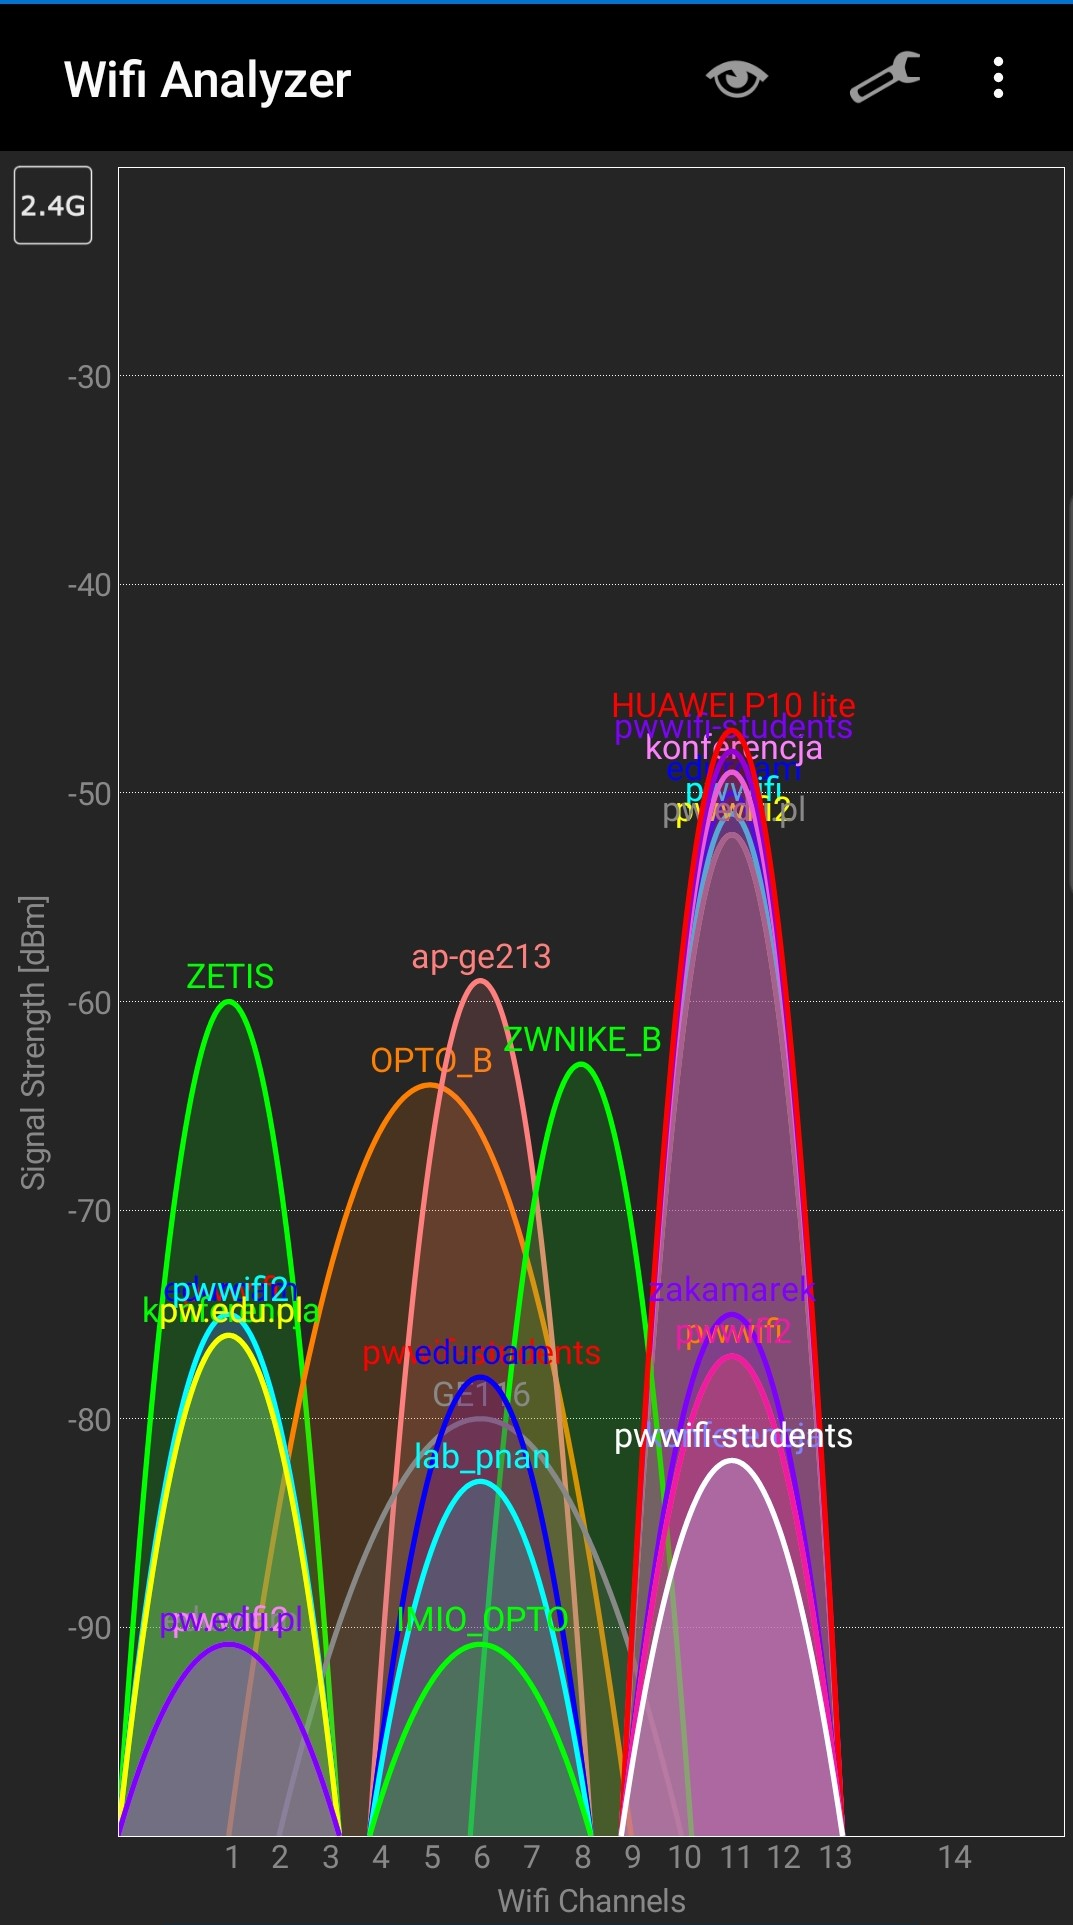
\includegraphics[width=0.4\textwidth]{Sieci-2,4GH}
%         \caption{Sieci na częstotliwości 2,4GHz}
%     \end{subfigure}
%     \begin{subfigure}[b]{0.49\textwidth}
%         \centering
%         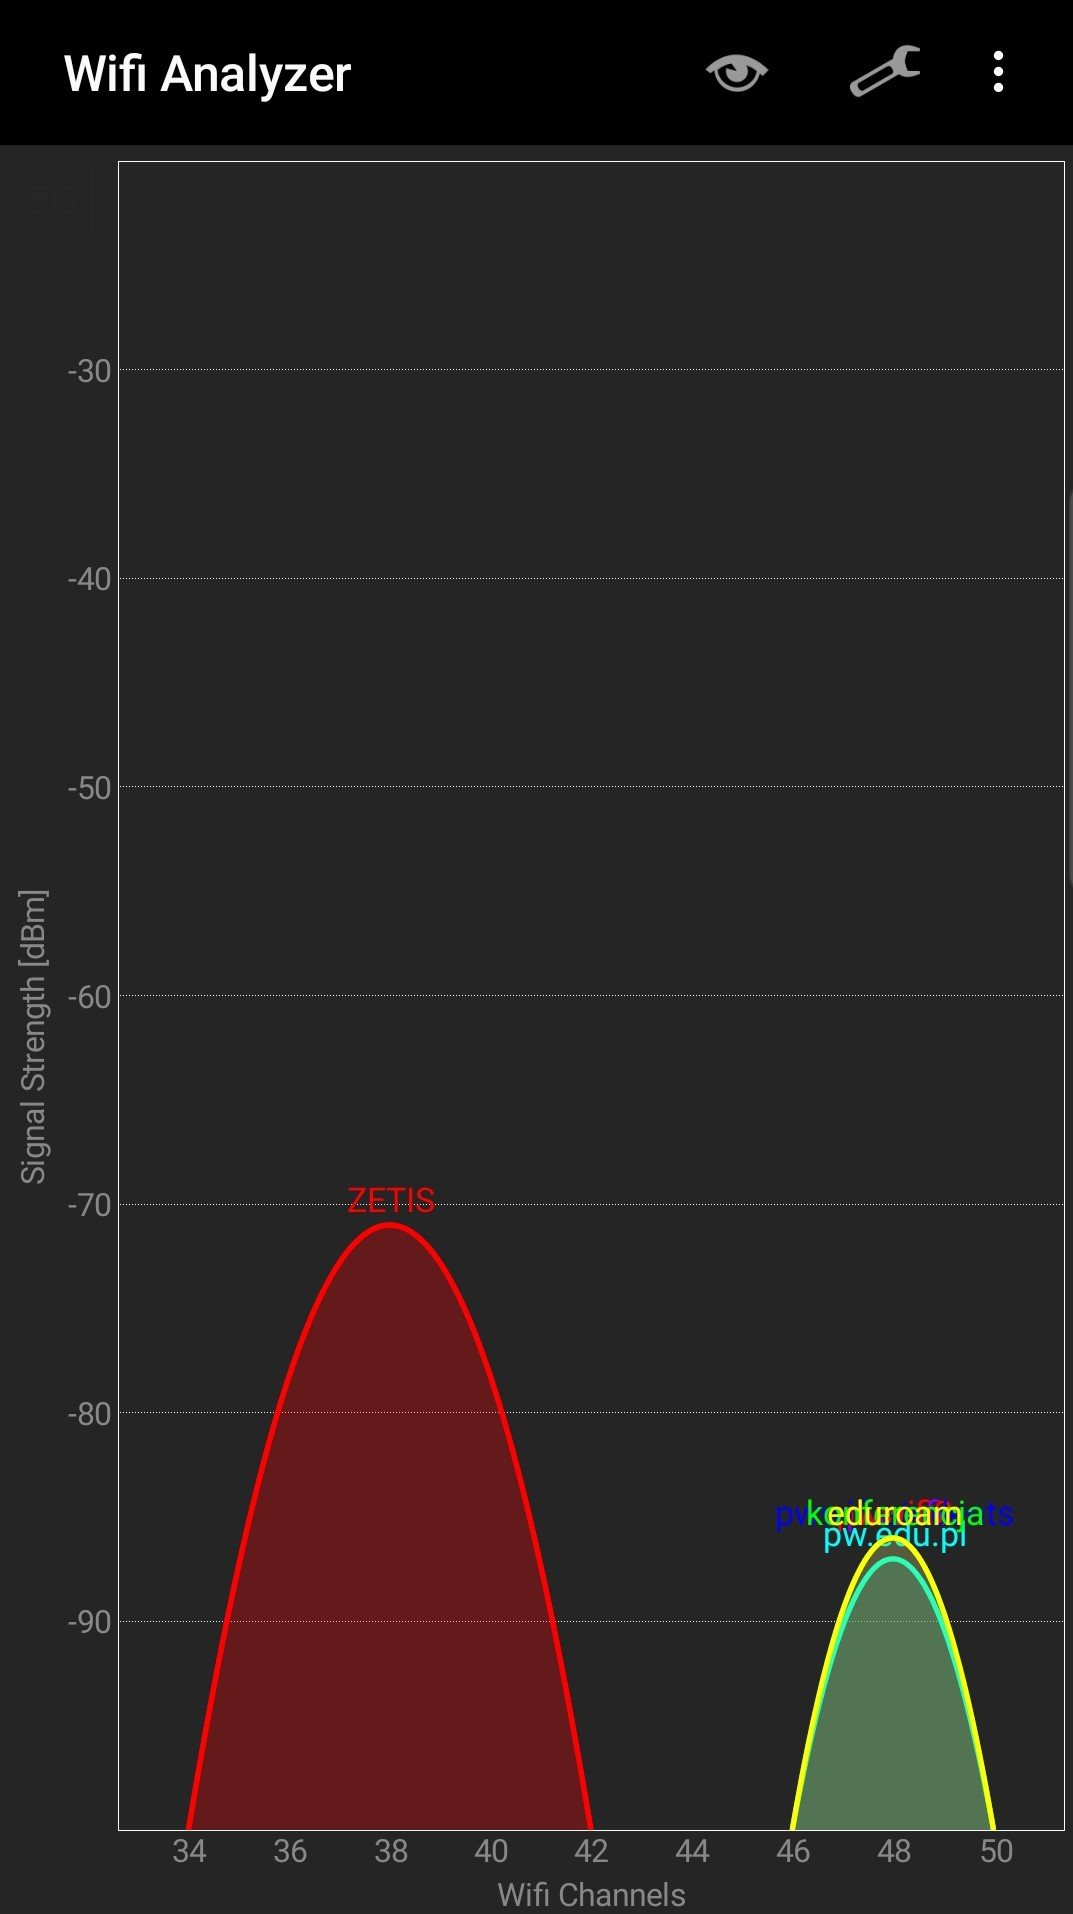
\includegraphics[width=0.4\textwidth]{Sieci-5GH}
%         \caption{Sieci na częstotliwości 5GHz}
%     \end{subfigure}
%     \label{fig:wifiAnalizer}
% \end{figure}

\section{Schemat sieci}
Strukturę urządzeń w sieci przedstawia rysunek \ref{fig:SchematSieci}.

\begin{figure}[H]
  \centering
  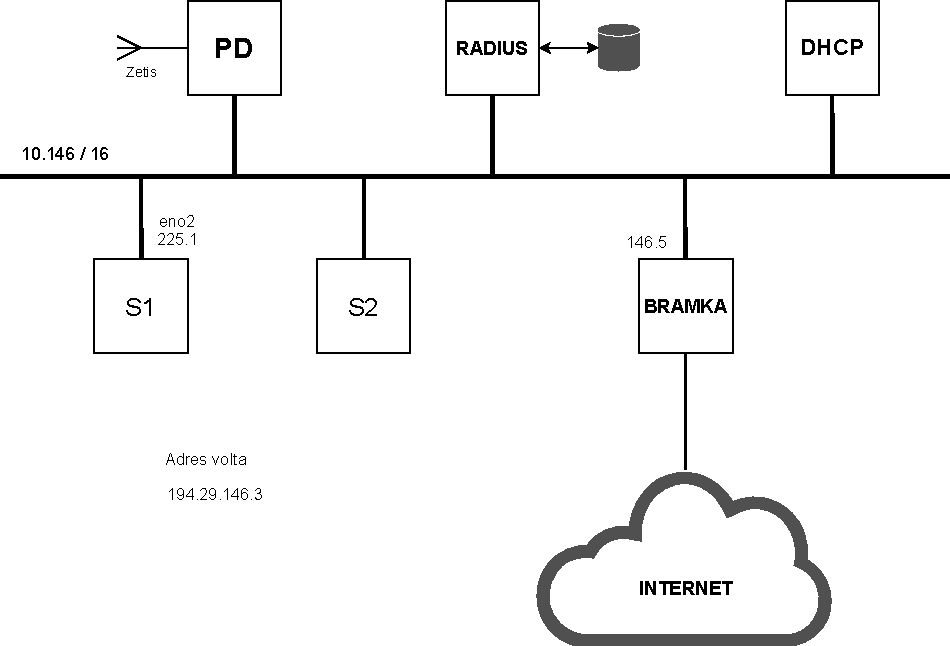
\includegraphics[width=\textwidth]{SchematSieci}
  
  \caption{Schemat sieci}
  \label{fig:SchematSieci}
\end{figure}

\section{Podłączenie do sieci wifi w środowisku graficznym}
W celu przyłączenia do sieci skorzystam z nakładki graficznej na program \textit{NetworkManager} wbudowanej w system Ubuntu.


\end{document}